\documentclass[a4paper,14pt]{extarticle}

\usepackage{graphicx}
\usepackage{xcolor}
\usepackage{mdframed}
\usepackage { amsmath , amssymb , amsthm }
\usepackage[T2A]{fontenc}
\usepackage[utf8]{inputenc}
\usepackage[english,russian]{babel}
\usepackage{tikz}
\usepackage{setspace}
\usepackage{mathtext}
\usepackage{float}
\usepackage[left=3cm, right=1cm, top=1.5cm, bottom=1.5cm]{geometry}
%\usepackage{icomma}
%\usepackage{indentfirst}
\usepackage{hyperref}

\graphicspath{{img/}}
\DeclareGraphicsExtensions{.pdf,.png,.jpg}
\singlespacing 

%\newenvironment{comment}{}{}

\begin{document}
\begin{titlepage}
  \begin{center}
    \MakeUppercase{Министерство науки и высшего образования Российской Федерации} \\
    \MakeUppercase{ФГБОУ ВО Алтайский госудаственный университет}
    \vspace{0.25cm}
    
    Институт цифровых технологий, электроники и физики
    
    Кафедра вычислительной техники и электроники
    \vfill
    
    {\LARGE Практика по получению первичных профессиональных умений и навыков}\\[5mm]
    \textsc{(Отчёт по практике направления подготовки бакалавров \\<<Информатика и вычислительная техника>>)}
  \bigskip

\end{center}
\vfill

\newlength{\ML}
\settowidth{\ML}{«\underline{\hspace{0.7cm}}» \underline{\hspace{2cm}}}
\hfill\begin{minipage}{0.4\textwidth}
  Выполнил студент 1-го курса, 595 группы:\\
  \underline{\hspace{\ML}} Д.\,В.~Осипенко\\
  «\underline{\hspace{0.7cm}}» \underline{\hspace{2cm}} \the\year~г.
\end{minipage}%
\bigskip

\hfill\begin{minipage}{0.4\textwidth}
  Проверил\\
  \underline{\hspace{\ML}} И.\,А.~Шмаков\\
  «\underline{\hspace{0.7cm}}» \underline{\hspace{2cm}} \the\year~г.
\end{minipage}%
\vfill

\begin{center}
  Барнаул, \the\year~г.
\end{center}
\end{titlepage}

\tableofcontents

\newpage

\section{01.06.2020}
Изучить и описать такие программы как: memtest,mhdd. Начать изучать основы работы с издательской системой TeX.
\subsection{Программа memtest}
Memtest\cite{MemTest86} - это бесплатная программа, загружаемая с USB, которая осуществляет тестирование RAM памяти компьютера на ошибки, используя серию комплексных алгоритмов и тестовых шаблонов.\\
\begin{center}
	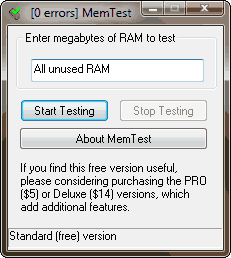
\includegraphics[scale=0.65]{img/memTest.png}
	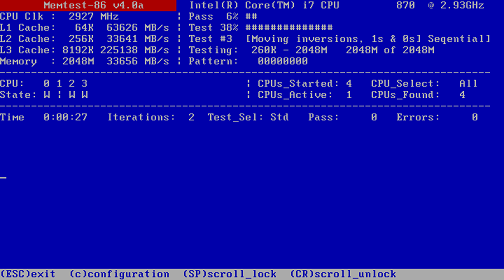
\includegraphics[scale=0.8]{img/Memtest86.png}\\ 
	Примеры программы memtest
\end{center}

Есть много хороших подходов для тестирования памяти. Однако многие тесты просто выбрасывают некоторые шаблоны в память, не задумываясь и не зная об архитектуре памяти или о том, как лучше всего обнаружить ошибки. Это хорошо работает для серьезных сбоев памяти, но мало помогает для поиска периодических ошибок. Тесты памяти на основе BIOS бесполезны для обнаружения периодических ошибок памяти. Микросхемы памяти состоят из большого массива плотно упакованных ячеек памяти, по одному на каждый бит данных. Подавляющее большинство периодических сбоев являются результатом взаимодействия этих ячеек памяти. Часто запись в ячейку памяти может привести к тому, что одна из соседних ячеек будет записана с одинаковыми данными. Эффективный тест памяти пытается проверить это условие. Поэтому идеальной стратегией для тестирования памяти было бы следующее:\\ \\
1. Написать ячейку с нулем\\
2. Записать все соседнии ячейки единицами, один или несколько раз\\
3. Проверить, что первая ячейка все еще нуль\\

Должно быть очевидно, что эта стратегия требует точного знания того, как ячейки памяти расположены на чипе. Кроме того, существует бесконечное число возможных схем размещения микросхем для различных типов микросхем и производителей, что делает эту стратегию неосуществимой. Однако существуют алгоритмы тестирования, которые могут приблизить этот идеал.\\

Memtest использует два алгоритма, значительно приближающие к идеальной стратегии тестирования. Первый называется <<moving inversions>>:\\ \\
1. Заполнить память по шаблону\\
2. Начать с меньшего адресса\\
 -Убедиться, что шаблон остался прежним\\
 -записать дополнение шаблона\\
 -увеличить адресс\\
 -повторить\\
3. Начать с наибольшего адресса
 -Убедиться, что шаблон остался прежним\\
 -записать дополнение шаблона\\
 -уменьшить адресс\\
 -повторить\\

Этот алгоритм хорошь в приближении к идеальному тесту памяти, но имеет свои недостатки. Кэширование, буферизация и выполнение не по порядку будет мешать данному алгоритму, из-за чего он будет менее эфективен. Чтобы устранить эти ограничения, был создан новый алгоритм <<Modulo-X>>. Этот алгоритм не зависит от кэша и буферизации:\\ \\
1. Для начального смещения 0-20\\
 -записать каждые 20ть локаций по шаблону\\
 -все другие локации записать дополнением шаблона\\
 -повторить 1 или несколько раз\\
 -проверить каждые 20ть локаций на соответствие шаблону\\

Этот алгоритм выполняет почти тотже уровень тестирования, что и приведенный ранее, но не подвержен кэшированию или буферезации.\\

Аналоги: Memtest86+, PassMark MemTest86, Windows Memory Diagnostic, GoldMemory, RAM Stress Test Pro2.
\newpage
\subsection{Программа mhdd}
MHDD\cite{real-world-systems} - это маленкая и в тоже время мощьная, бесплатно распространяемая утилита для работы с жесткими дисками на наиболее низком уровне из возможных. Первая версия была выпущена в 2000 году Дмитрием Постриганом, целью которого было создать понятную и надежную программу для диагностики. 
\begin{center}
	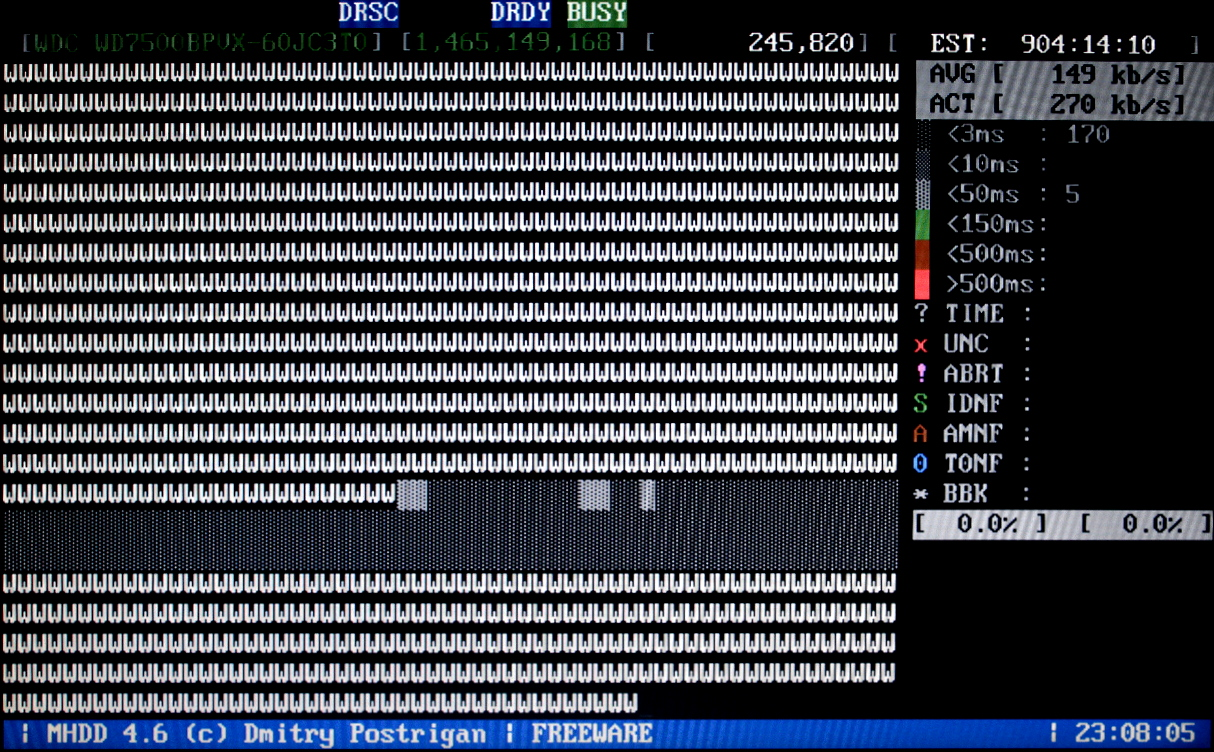
\includegraphics[scale=0.3]{img/mhdd1.png}\\
	\vspace{0.25cm}
	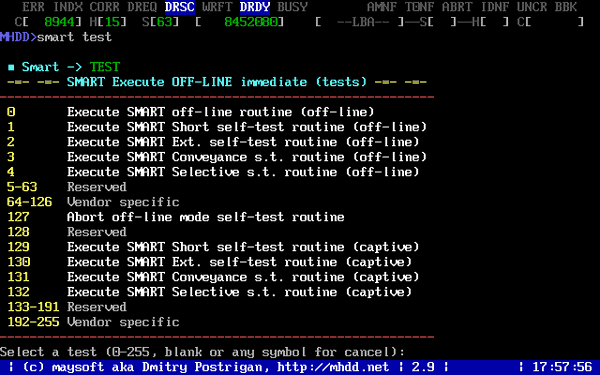
\includegraphics[scale=0.81]{img/mhdd2.png}\\
	Примеры работы программы mhdd
\end{center}

Когда DOS необходимо считать сектор с диска, он просит BIOS сделать это. BIOS смотрит его таблицы пытаясь найти где этот диск подключен, проверяет диапазоны и после начинает отправлять команды на диск. Когда все сделанно BIOS возвращает результаты в DOS.\\

MHDD не использует функции DOS или BIOS, и работает даже если система не обнаруживает диск. MHDD работает напрямую с IDE или контролером Serial ATA.

Аналоги: HDDlife,Victoria HDD,HDD Recovery Pro.
\newpage
\section{02.06.2020}
Изучить и описать работу следующих программы как: Clonezilla, DD из GNU coreutils. Начать оформление отчёта.
\subsection{Программа Clonezilla}
Clonezilla\cite{clonezilla} - это программа для создания разделов и клонирования дисков. Она помогает развертывать систему, выполнять резервное копирование и восстановление с нуля. Программа сохраняет и восстанавливает только использованные блоки на жестком диске.
\begin{center}
  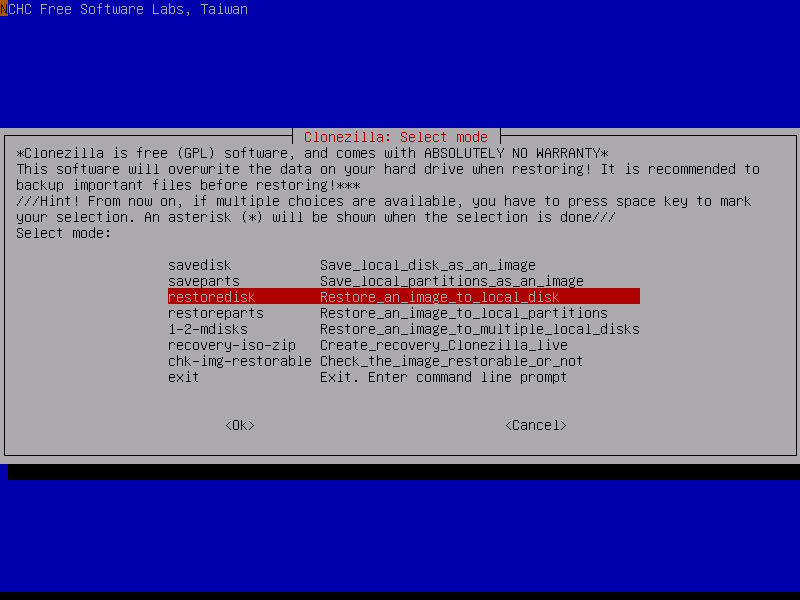
\includegraphics[scale=0.6]{img/Clonezilla1.png}\\
  Пример программы Clonezilla
\end{center}
Особенности:\\
- Поддержка многих файловых систем\\
- Boot loader, включая grub и syslinux\\
- Возможность зашифровать образ\\
- Распространяется по лицензии GNU v2\\
и др.\\ \\
Ограничения:\\
- Целевой раздел должен быть больше или равен размеру исходного\\
- Не реализованны функции онлайн клонирования, дифференциального резервного копирования\\
- Образ не может быть исследован или смонтирован
\subsection{dd из GNU coreutils}
dd(dataset definition) - это утилита, позволяющая копировать файлы из стандартного потока с изменяемых входным/выходным размеров блока, при желании выполняя преобразования на нем
\begin{center}
  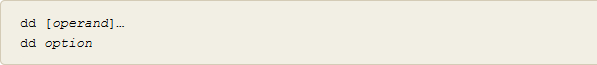
\includegraphics{img/dd.png}
\end{center}
Имеет только две опции : --help и --version. В наличии ОГРОМНЫЙ список параметров, который можно мосмотреть на официальном сайте\cite{gnu-dd}
\newpage
\section{03.06.2020}
Изучить следующие понятия: виртуализация, эмуляция, аппаратная виртуализация, гипервизор. Продолжить оформление отчёта.
\subsection{Виртуализация}
Вертуализация\cite{virt} - это технология, позволяющая вам создать ИТ сервит используя ресурсы, привязанные к железу. Она дает возможность использовать одну машину в полном объеме, разделяя ее ресурсы на множество пользователей или сред
\begin{center}
  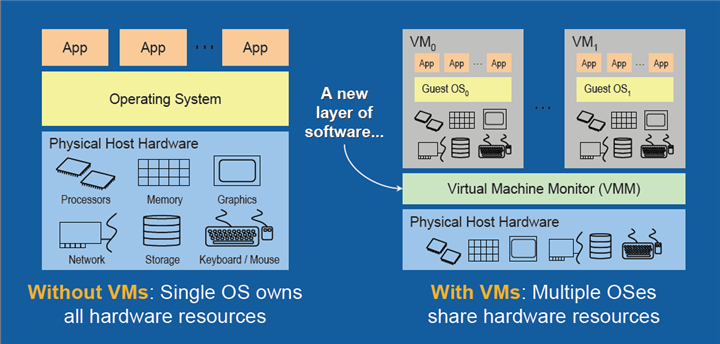
\includegraphics{img/virtualization.png}
\end{center}
Программа называемая hypervisors разделяет физическиее ресурсы от виртальных сред - вещей, которым нужны эти ресурсы. Hypervisors могут находится поверх OS или устанавливаться непосредственно на оборудование. Эта программа берет ваши физические ресерсы и разделяет их между виртуальными средами, которые могут использовать их. Когда виртульное окружение работает и пользователь или программа запрашивает больше ресурсов от железа, hypervisor передает запрос физической системе и кэширует изменения.\\
\begin{center}
  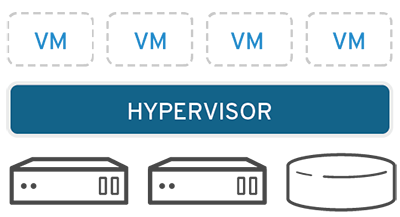
\includegraphics[scale=0.7]{img/how-virtualization-works.png}\\
\end{center}
Виды виртуализации:\\
1) Data virtualization - множество данных может быть объеденено в один источник\\
2) Desktop virtualization - позволяет сис.админу развернуть образы рабочего стола на сотни физических машин\\
3)Server virtualization - позволяет серверу выполнять больше специфичных для него операций и функций.\\
4)OS virtualization - возможность запускать две OS рядом друг с другом.\\
\newpage
\section{04.06.2020}
Установить и настроить VirtualBoX (или другую систему виртуализации), описать процесс установки и настройки программы.
\subsection{Процесс установки virtualbox}
Скачаваем исполняемый файл с официального сайта virtualbox\cite{virtualbox} и запускаем его. Начинается подготовка к установке, затем появляется окно выбора того, что установится и куда. Выбираем что нужно и нажимаем "далее". В открывшемся окне (рисунок 4) будет предложены базовые настройки запуска виртуальной машины:\\
- создать ярлык на рабочем столе;\\
- создать ярлык в панели быстрого запуска;\\
- зарегистрировать расширения файлов Virtual Box в операционной системе.\\
\begin{center}
  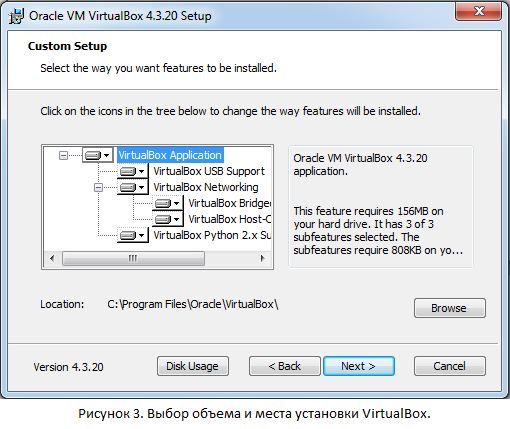
\includegraphics[scale=0.465]{img/VirtualBox1.png}
  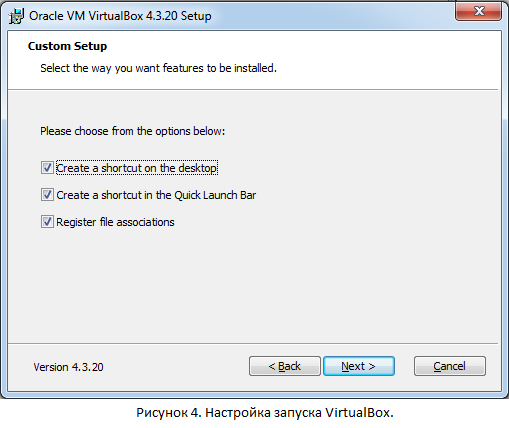
\includegraphics[scale=0.465]{img/VirtualBox2.png}\\
\end{center}
Затем два раза жмем "далее" и начинается установка программы. После этого завершаем установку.
\begin{center}
  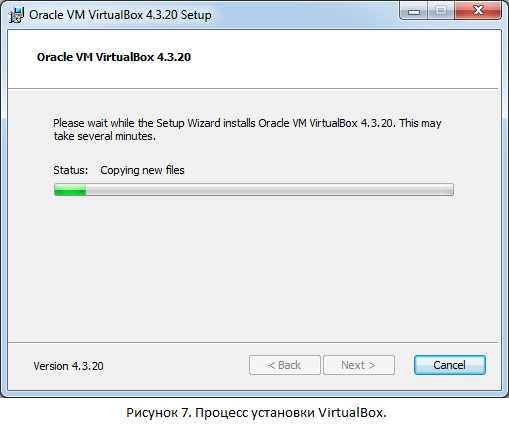
\includegraphics[scale=0.465]{img/VirtualBox3.png}
  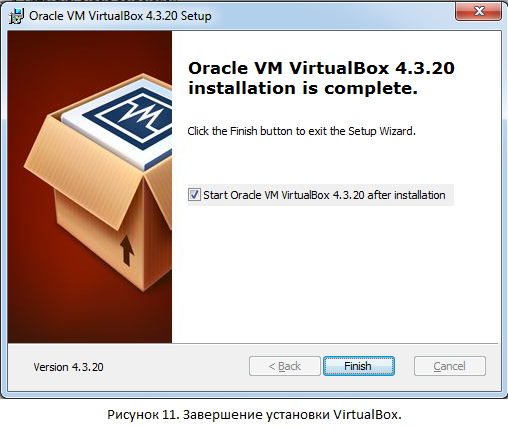
\includegraphics[scale=0.465]{img/VirtualBox4.png}
\end{center}
\newpage
\section{05.06.2020}
Установить FreeDos на виртуальную машину, описать процесс установки, осуществить запуск и проверку работоспособности системы.
\subsection{Установка FreeDos}
Скачиваем образ диска с официального сайта FreeDos\cite{freedos} и создаем образ машины
\begin{center}
  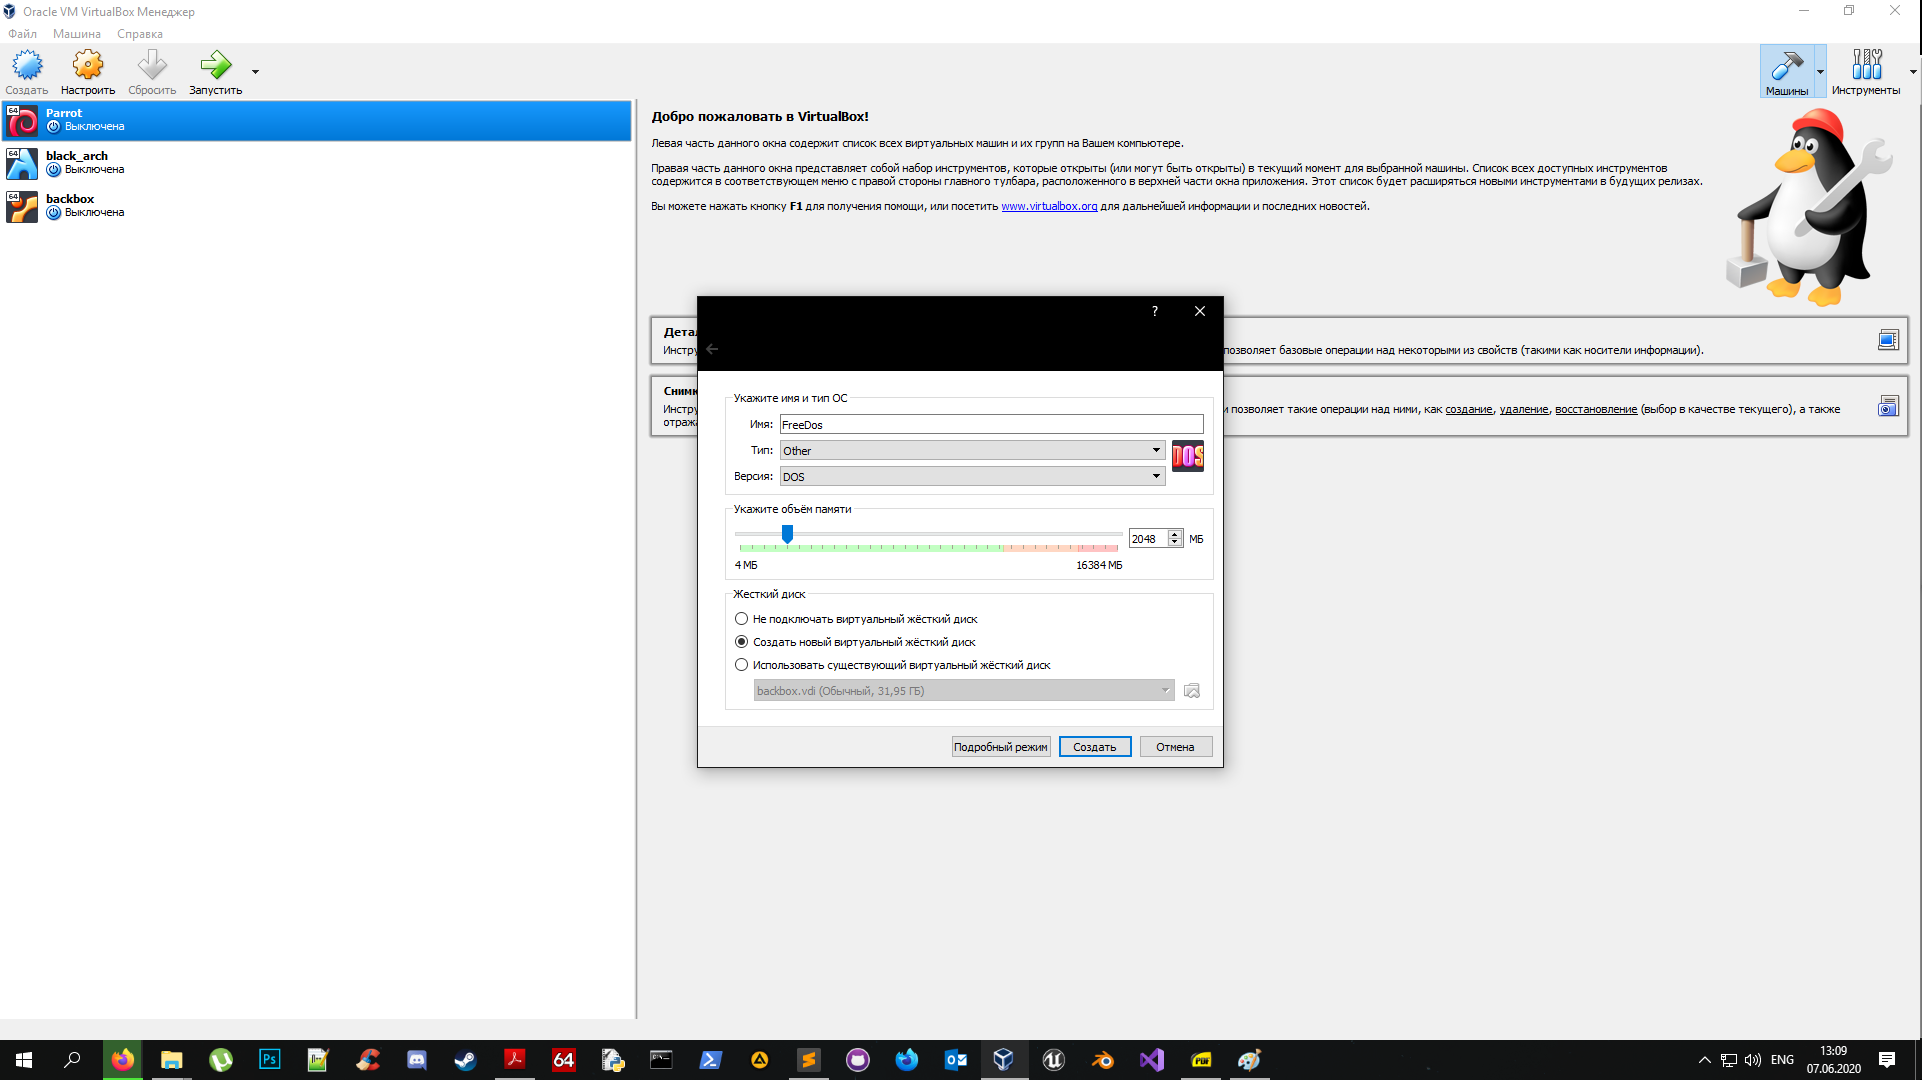
\includegraphics[scale=0.3]{img/Freedos1.png}
\end{center}
Начинаем установку, соглашаемся со всем, жмем далее и ждем ее окончания установки.
Но так как мой BIOS не подходит для FreeDos, то я не могу его установить и следовательно проверить работаспособность.
\newpage
\section{06.06.2020}
Установить Debian GNU/Linux на виртуальную машину:\\
-установку производить в режиме netinstall;\\
-использовать LVM, название тома фамилия на английском;\\
-установить openssh-server;\\

Изучить понятие LVM. Осуществить доступ к виртуальной машине по протоколу SSH (например ssh или putty).
\section{08.06.2020}
Установить в виртуальной машине следующие пакеты:\\
        1)openssh-server;\\
        2)rsync;\\
        3)scalpel;\\
        4)gddrescue.\\

Изучить, для чего используются данные программы. Познакомиться с FAT (File Allocation Table «таблица размещения файлов») и её версиями (FAT12 / FAT16 / FAT32).
\section{09.06.2020}
Познакомиться с файловыми системами и описать:\\
        -extX (где X версия);\\
        -NTFS;\\
        -Btrfs;\\
        -NFS.\\ \\       
Изучить такие таблицы разделов как:\\
        -MBR;\\
        -GPT.\\
\newpage
\section{10.06.2020}
Изучить базовые основы сетевой фильтрации пакетов в следующих программах:\\
        -nftables (используется в Debian Buster GNU/Linux по умолчанию);\\
        -брандмауэр Windows Defender.\\

Описать защиту устройства с помощью следующих программ и действий:\\
        -разграничение прав доступа;\\
        -clamav;\\
        -Dr.Web;\\
        -Kaspersky Antivirus (KAV).\\
\subsection{Разграничение прав доступа}
- позваляет предотвратить несанкционированный доступ к важным и системным файлам или порчу самой системы.
\subsection{clamav}
- это open source антивирусный набор инструментов, использующаяся в различных ситуациях, включая сканирования электронной почты, веб сканирования.

Он предоставляет ряд утилит, включая гибкий и масштабируемый многопоточный демон, сканер командной строки и расширенный инструмент для автоматического обновления баз данных. Ядром пакета является антивирусный движок, доступное в форме распространяемой библиотеки.\cite{clamav}
\subsection{Dr.Web}
- российский разработчик антивирусных программ и сервисов для предоставления услуг информационной защиты

Компонент используется для доступа к любым объектам файловой системы (файлы, каталоги, загрузочные записи). Запускается с правами суперпользователя root.

Индексирует все проверенные файлы и каталоги и сохраняет данные о проверенных объектах в специальном кэше, чтобы не выполнять повторную проверку объектов, которые уже были проверены ранее и не изменялись с момента последней проверки (в этом случае, если заявка о проверке такого объекта поступает повторно, возвращается результат его предыдущей проверки, извлеченный из кэша). Схема работы компонента показана на рисунке ниже.

\begin{center}
  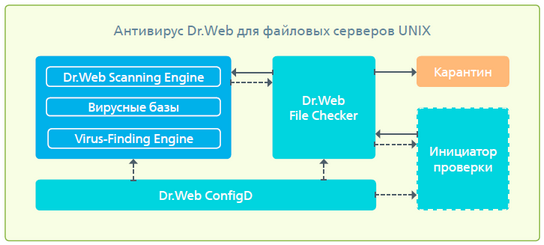
\includegraphics[scale=0.9]{img/drweb.png}
\end{center}
При поступлении запросов на проверку объектов файловой системы от компонентов программного комплекса Dr.Web для файловых серверов UNIX проверяет, требуется ли проверка запрошенного объекта, и если да, то формирует задание на проверку его содержимого для сканирующего ядра Dr.Web Scanning Engine. В случае если проверенный объект содержал угрозу, то компонент проверки файлов Dr.Web File Checker применяет к нему нейтрализующее действие (удаление или перемещение в карантин), в случае если это действие задано клиентским компонентом, инициировавшим проверку, в качестве реакции на угрозу. В качестве инициаторов проверки могут выступать различные компоненты продукта (например, монитор SpIDer Guard для SMB).

В процессе проверки запрошенных объектов файловой системы компонент проверки файлов формирует и отправляет компоненту-клиенту, запросившему проверку, отчеты о результатах проверки и предпринятых действиях по нейтрализации угроз, если они были обнаружены.

Помимо стандартного метода проверки файлов, для внутренних нужд поддерживаются специальные методы проверки файлов:

•Метод «flow» – метод потоковой проверки файлов. Компонент, использующий данный метод, один раз инициализирует параметры проверки и обезвреживания угроз, и далее эти параметры будут применяться ко всему потоку заявок на проверку файлов, поступающих от компонента. Этот метод проверки используется монитором SpIDer Guard.

•Метод «proxy» – метод проверки файлов, заключающийся в том, что компонент проверки файлов выполняет только проверку файлов на наличие угроз, не применяя к ним никаких действий, в том числе не выполняя регистрацию обнаруженных угроз (эти действия целиком возлагаются на компонент, инициировавший проверку). Этот метод проверки используется монитором SpIDer Guard для SMB и компонентом Dr.Web ClamD.

Имеется возможность проверить файлы с использованием методов «flow» и «proxy», используя команды flowscan и proxyscan утилиты Dr.Web Ctl (запускается командой drweb-ctl), однако для обычной проверки файлов по требованию рекомендуется использовать только команду scan.

В процессе своей работы компонент проверки файлов собирает общую статистику проверки файлов, усредняя количество файлов, проверенных в течение секунды за последнюю минуту, последние 5 минут, последние 15 минут.\cite{drweb}


\subsection{Kaspersky Antivirus}
- антивирусная программа, разработанная «Лабораторией Касперского» Он предназначен для защиты пользователей от вредоносных программ.

Работа различных антивирусов одного класса мало чем отличается. Антивирус Касперского обеспечивает защиту среднего класса, поскольку не контролирует сетевой трафик в полном объеме. Работает антивирус так. В течении всего времени, когда компьютер включен он следит за запускаемыми программами, подключаемыми внешними устройствами и скачиваемыми файлами. При запуске программы Антивирус Касперского оценивает ее безопасность еще до исполнения кода. Таким образом он пытается заблокировать вредоносное ПО прежде чем оно успеет навредить вашему компьютеру. 

Антивирусное сканирование всей системы нужно применить сразу после установки антивируса. После сканирования вы будете уверены в том, что ваша система чиста. Такие проверки можно выполнять автоматически с определенной периодичностью. Антивирус будет выполнять их сам, вам нужно лишь настроить частоту.

Почтовый и IM модули программы работаю, соответственно с email – и IM-клиентами. То есть программами с помощью которых вы просматриваете почту и с помощью которых обмениваетесь сообщениями. В этих программах блокируются вредоносные ссылки и зараженные прикрепленные файлы. 

Если антивирус находит вредоносную программу или файл, то он действует по правилам, установленным в настройках. Как правило – это автоматическое удаление файла, или перемещение его в карантин, но вы можете настроить реакцию антивируса более точно.

Kaspersky Anti-Virus требует определенных ресурсов компьютера, но не загружает систему критически. Кроме того, есть Игровой режим, при активации которого антивирус прекращает все свои ресурсоемкие операции и передает всю мощность компьютера игре. В Игровом Режиме не выводятся сообщения, чтобы вас не тревожить.\cite{kasav}
\newpage
\section{11.06.2020}
Клонировать виртуальную машину с Debian Buster GNU/Linux, и проделать следующие действия:\\
        -создать текстовый файл и перебросить его с одной машину на другую, с помощью rsync;\\
        -осуществить доступ по ключу (потребуется как этап, команда: ssh-keygen) с одной виртуальной машины на другую.\\

Использовать пакет mtools (команда mformat) создать файл-образ на 1 Mb, с файловой системой FAT32 и выполнить следующие действия:\\
        -подключить данный файл с помощью команды mount (от root);\\
        -добавить текстовый файл с выводом следующих команд: pvs, vgs, lvs, название файла ФамилияИО.txt (латиницей).\\

Посмотреть базовые ключи команды debugfs.
\section{Выводы по проделанной работе}
В ходе данной практики были выполнены большинство поставленных задач и полученно немножечко навыков использования современных информационных технологий.  Это все что можно сказать про данную практику.\\

Думаю в следующий раз лучше ставить более конкретные цели на практику, чем те, что были представленны в этот раз.
\newpage
\begin{thebibliography}{}
	\bibitem{MemTest86}
	\url{https://www.memtest86.com/tech_memtest-algoritm.html}
	\bibitem{real-world-systems}
	\url{http://real-world-systems.com/docs/MHDD_en_manual.html}
	\bibitem{xakep}
	\url{https://xakep.ru/2016/11/08/mhdd/}
  \bibitem{clonezilla}
  \url{https://clonezilla.org/}
  \bibitem{gnu-dd}
  \url{https://www.gnu.org/software/coreutils/manual/html_node/dd-invocation.html}
  \bibitem{virt}
  \url{https://www.redhat.com/en/topics/virtualization/what-is-virtualization}
  \bibitem{virtualbox}
  \url{https://www.virtualbox.org/wiki/Downloads}
  \bibitem{freedos}
  \url{https://www.freedos.org/download/}
  \bibitem{clamav}
  \url{https://www.clamav.net/documents}
  \bibitem{drweb}
  \url{https://download.geo.drweb.com/pub/drweb/unix/server/10.0/documentation/html/ru/index.html?dw_9_filecheck_principles.htm}
  \bibitem{kasav}
  \url{https://howto.mydiv.net/view-Kak-rabotaet-Antivirus-Kasperskogo.html}
\end{thebibliography}

\newpage
\end{document}
 